\section{Selección del Modelo de Suavizado}
En esta sección se aplican diferentes métodos de suavizado para analizar la evolución de la serie temporal. Algunos modelos fueron descartados previamente, ya que no se ajustaban a las características de la serie en estudio.\\

El \textbf{modelo de alisado simple} fue descartado, ya que está diseñado para series sin tendencia ni estacionalidad. Dado que la serie presenta ambos componentes, este método resulta inadecuado.\\

El \textbf{modelo de alisado doble} permite modelar la tendencia, pero no la estacionalidad. Dado que nuestra serie exhibe un comportamiento estacional, este método también fue descartado.\\

Finalmente, el \textbf{modelo de alisado Holt-Winters} fue seleccionado, ya que es el más adecuado para series con con tendencia y estacionalidad.

\subsection{Modelo Holt-Winters}
Para crear el modelo de Holt-Winters en Python se utiliza el siguiente código:
\begin{lstlisting}
	modelo_holt_winters = sm.tsa.ExponentialSmoothing(train_TR["Sales"], trend = "add",
	seasonal = "additive", seasonal_periods = 7).fit()
	predicciones_hw = modelo_holt_winters.forecast(steps = 20)
	modelo_holt_winters.summary()
\end{lstlisting}

Los parámetros para la función \lstinline|sm.tsa.ExponentialSmoothing| se escogieron utilizando el siguiente criterio:
\begin{itemize}
	\item \textbf{train\_TR["Sales"]}: son los datos de entrenamiento.
	\item \textbf{trend="add"}: indica que la tendencia se ajusta de forma aditiva, es decir, el crecimiento de la serie en el tiempo se modela sumando un valor constante en cada período. La tendencia presenta un movimiento lineal, en vez de parabolico.
	\item \textbf{seasonal="additive"}: modela la estacionalidad de forma aditiva. Se ha elegido dado que la amplitud de la estacionalidad es aproximadamente constante a lo largo del tiempo.
	\item \textbf{seasonal\_periods=7}: se observa que los períodos estacionales suelen repetirse aproximadamente cada 7 días, es decir, muestra una estacionalidad semanal. 
\end{itemize}

Para hacer el $forecast()$ se escogio un step de $20$. Este número representa 20 días, justamente la cantidad reservada en el conjunto de datos de test. La siguiente figura muestra el conjunto observado, el test y el modelo Holt-Winters.\begin{figure}[h]
	\centering
	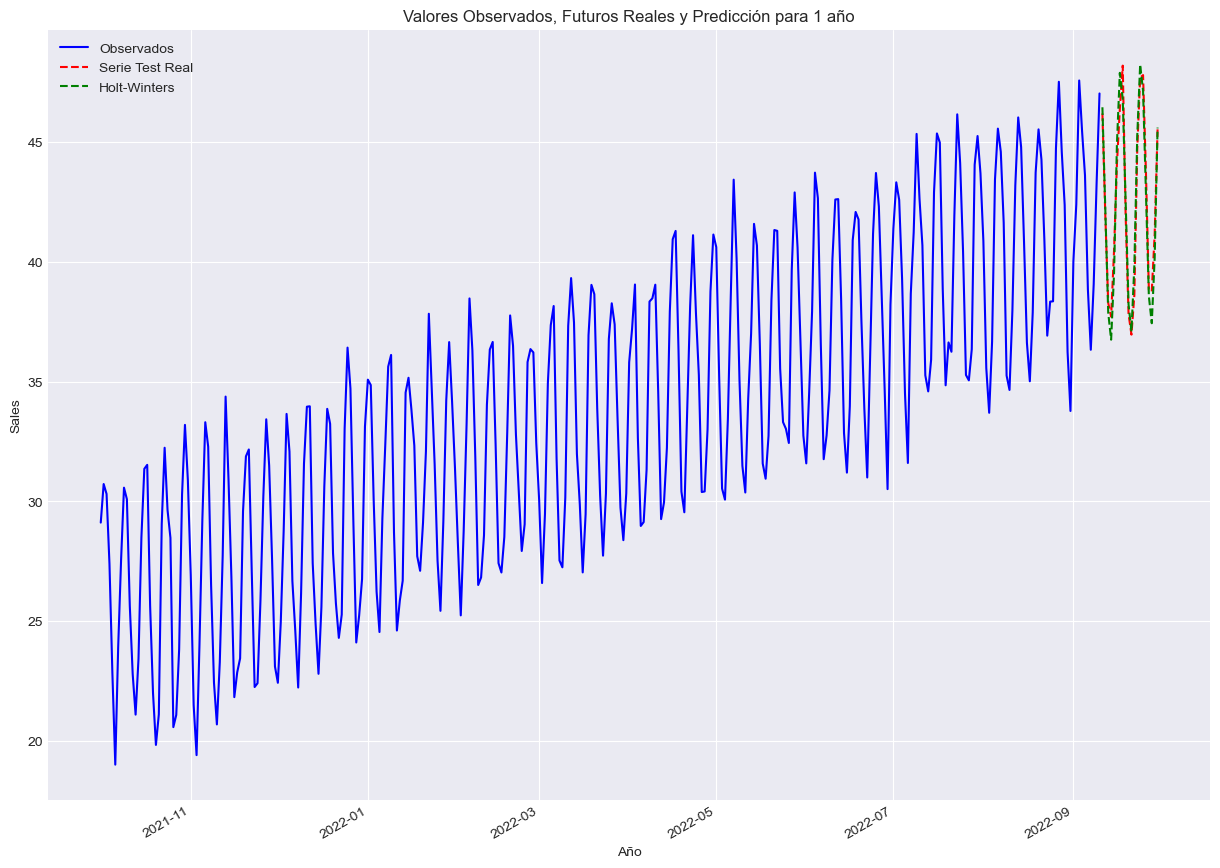
\includegraphics[width=0.7\linewidth]{modelo_holt_wunters}
	\caption{Gráfico Modelo Holt-Winters}
	\label{fig:modeloholtwunters}
\end{figure}

\subsubsection{Errores del Modelo}

Para evaluar la precisión del modelo de predicción se calcularon el error absoluto y el error absoluto medio (MAE). La siguiente figura muestra la evolución del valor del error absoluto por día.
\begin{figure}
	\centering
	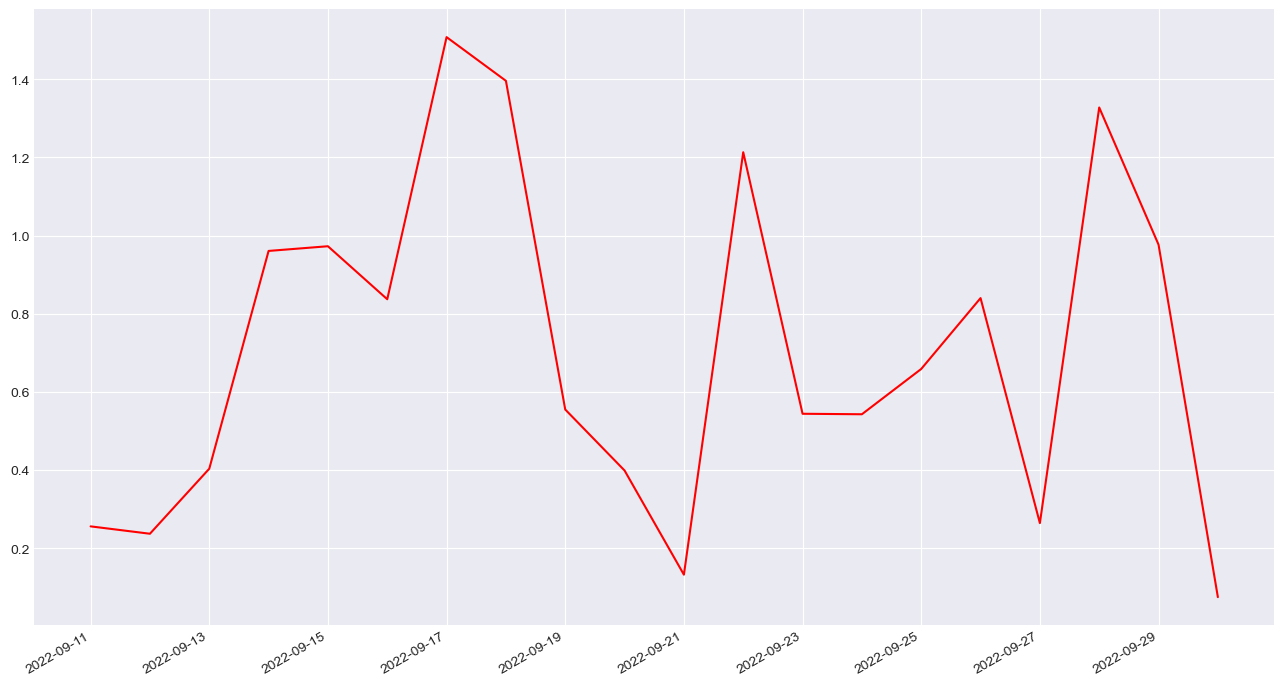
\includegraphics[width=0.7\linewidth]{errores_diarios_test_prediccion}
	\caption{Gráfico Error Valor Absoluto por Día}
	\label{fig:erroresdiariostestprediccion}
\end{figure}
	
Se obtiene el error absoluto medio para el modelo: $0.70488$. So consideramos que el valor medio de $Sales$ en el conjunto $test$ es de 45, este error representa aproximadamente 1,58\%, lo que indica un buen desempeño en térmminos relativos.

\subsubsection{Transformación Logarítmica}
Para mejorar la estabilidad de la serie temporal, se aplicó una transformación logarítmica, cuyo objetivo principal es reducir la heterocedasticidad, la variabilidad no constante, y hacer que la serie sea más adecuada para modelos aditivos. Esta transformación es especialmente útil cuando la amplitud de la estacionalidad crece con el tiempo. \\

Además, se aplicó una diferenciación a la serie logarítmica, un proceso que permite eliminar tendencias de largo plazo y convertir la serie en estacionaria, una propiedad fundamental para muchos modelos de series temporales, incluidos los métodos de suavizamiento exponencial como Holt-Winters. El siguiente código muestra los pasos realizados. Los parámetros utilizados son los mismo que en el primer modelo de Holt-Winters.
\begin{lstlisting}
	train_log = np.log(train_TR['Sales'])
	train_log_diff = train_log.diff().dropna()
	modelo_hw_diff = sm.tsa.ExponentialSmoothing(train_log_diff, trend='add',
	 seasonal='add', seasonal_periods=7).fit()
	pred_diff = modelo_hw_diff.forecast(steps=20)
\end{lstlisting}
Una vez obtenidas las predicciones en la escala logarítmica diferenciada, es necesario reconstruir la serie original. Para ello, se revierte la diferenciación acumulando los valores predichos y se aplica la exponenciación para deshacer la transformación logarítmica.
\begin{lstlisting}
	last_log_value = train_log.iloc[-1]  
	pred_log = last_log_value + pred_diff.cumsum()
	pred_final = np.exp(pred_log)
\end{lstlisting}

Realizar la combinación de transformación logarítmica, diferenciación y el modelo Holt-Winters permitió generar predicciones con una baja tasa de error, asegurando que la serie sea más estable y adecuada para el análisis. 

La siguiente figura muestra la comparación entre el modelo logarítmico y el modelo básico frente a los datos del conjunto de prueba.\\

Ambos modelos presentan un comportamiento muy similar; sin embargo, se observa que el modelo logarítmico se extiende más en la parte inferior, lo que sugiere una mejor cobertura de los márgenes de error.
\begin{figure}[h]
	\centering
	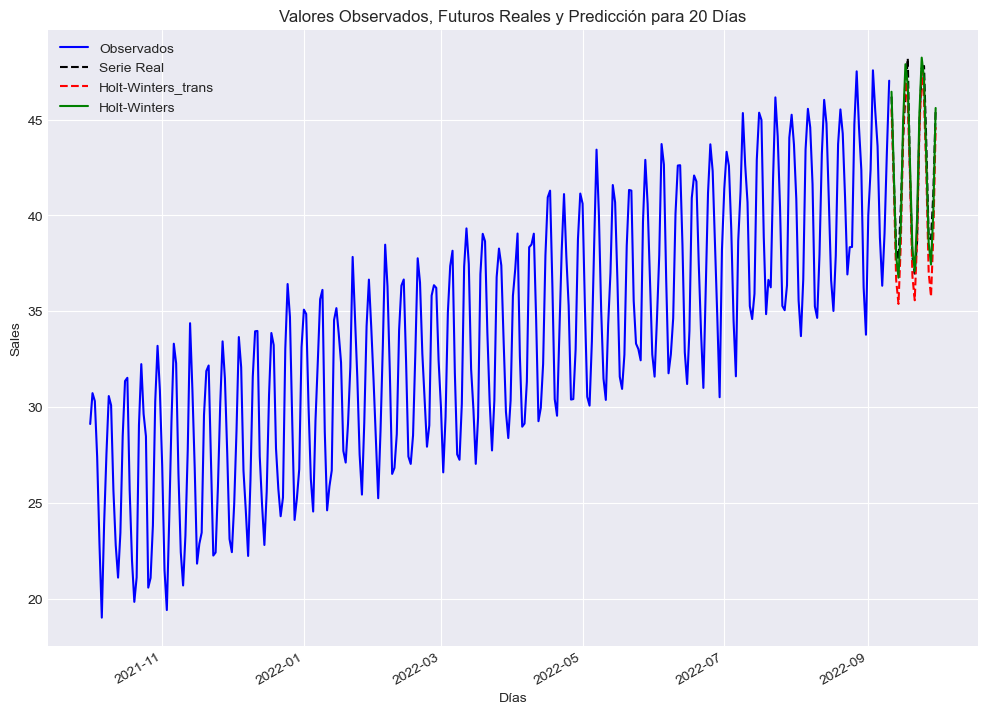
\includegraphics[width=0.7\linewidth]{holt_winters_log}
	\caption{Gráfico de Holt-Winters-Trans}
	\label{fig:holtwinterslog}
\end{figure}

\subsection{Errores del Modelo de Transformación Logarítmica}
Se evalua de la misma forma que para el modelo original. Se obtiene un MAE de 1.228. Esto representaría un error del 2,79\%.

